%Beamer class
\documentclass{beamer}

\usepackage[czech]{babel}
\usepackage[cp1250]{inputenc}
\usepackage{fontenc}
\usepackage{tgheros}
\usepackage{array}
\usepackage{color}
\usepackage{hyperref}

\usetheme{Antibes}
\usecolortheme{crane}


\title[BE1M13VES]{BE1M13VES}
\subtitle[Manufacturing of Electrical Components] {Manufacturing of Electrical Components}
\author[Brejcha]{Michal Brejcha}
\institute[CTU]{CTU in Prague}
\date[Prague, 2017]{Prague, 2017}

\begin{document}
%------------------------------------------------------------------------------
%Uvodni slajd
%------------------------------------------------------------------------------
\frame{\titlepage}

\begin{frame}
\frametitle{Overview} 
\tableofcontents
\end{frame}

\AtBeginSection[]
{
  \begin{frame}
    \frametitle{TOPIC}
    \tableofcontents[currentsection]
  \end{frame}
}

%------------------------------------------------------------------------------
%Frquency dependency of resistors
%------------------------------------------------------------------------------
\section{\texorpdfstring{Frequency dependency of resistors}{Frequency dependency of resistors}}
%------------------------------------------------------------------------------
	\begin{frame}
    \frametitle{Equivalent Circuit}
		
		For AC circuits the parasitic serial inductance and parallel capacity must be taken into account. The frequency dependence of the resistors is caused especially by its construction.
		\begin{center}
			\begin{tabular}{m{0.45\linewidth} m{0.45\linewidth}}
			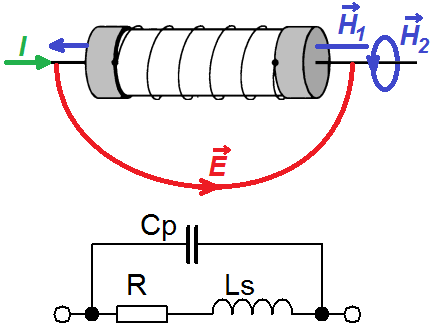
\includegraphics[scale=0.4]{obr01_poleRes.png} &
			
			\begin{itemize}
				\item $H_1$, $H_2$... magnetic field from resistive track and leads.
				\item $E$... electric field (capacitance) between opposite sides of package and leads.
			\end{itemize}
			\end{tabular}
		\end{center}
	\end{frame}
%------------------------------------------------------------------------------
	\begin{frame}
    \frametitle{Technology Overview}
		
		\begin{itemize}
			\item Parasitic capacitance is dominant for higher values of resistance ($>$k$\Omega$).
			\item Parasitic inductance is dominant only for small values of resistance ($<$100$\Omega$) and frequencies smaller than resonant frequency.
			\item Larger packages have larger parasitic inductance
			
			\begin{itemize}
				\item power resistors (resistive wire) - worst
				\item small smd thin film resistors - best
			\end{itemize}
			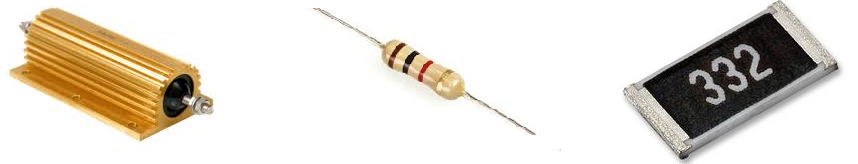
\includegraphics[scale=0.4]{obr05_technR.png}
		\end{itemize}
	\end{frame}
%------------------------------------------------------------------------------
	\begin{frame}
    \frametitle{Impedance Plot Example}

		\begin{center}
			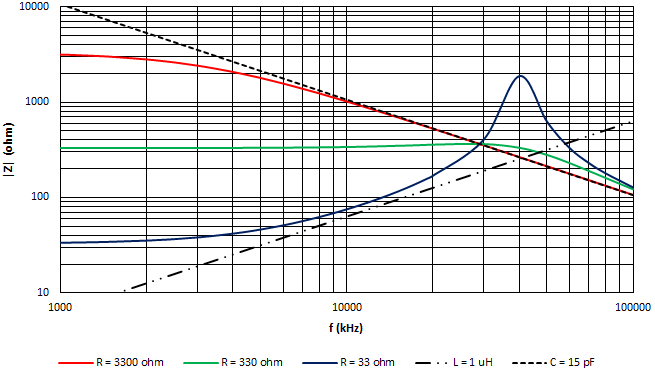
\includegraphics[scale=0.62]{obr02_impedanceR.png}
		\end{center}
	\end{frame}
%------------------------------------------------------------------------------
	\begin{frame}
    \frametitle{Equivalent Circuit Analysis}
		Impedance: 
		$$\hat{Z}= \frac{R - \frac{j}{\omega C_p}\cdot\left(\omega^2 L_sC_p\cdot\left(\omega^2 L_sC_p - 1\right)+\left(\omega C_pR\right)^2\right)}{\left(1-\omega^2 L_sC_p\right)^2+\left(\omega C_pR\right)^2}$$
		Low frequencies ($\omega \rightarrow 0$): \textcolor{red}{resistivity}
		$$\hat{Z}\approx R$$
		High frequencies ($\omega >> \omega_{RES}$): \textcolor{red}{parasitic capacitance effect}
		$$\hat{Z}\approx \frac{1}{j\omega C_p}$$
	\end{frame}
%------------------------------------------------------------------------------
	\begin{frame}
    \frametitle{Equivalent Circuit Analysis - Resonance}
		Resonance frequency:
		$$\omega_{RES}= \sqrt{\frac{1}{L_sC_p} - \left(\frac{R}{L_s}\right)^2}$$
		Impedance at $\omega_{RES}$
		$$\hat{Z}_{RES}=\frac{Z_0^2}{R}$$
		Where $Z_0$ has the same definition as wave impedance:
		$$Z_0 = \sqrt{\frac{L_s}{C_p}}$$
	\end{frame}
%------------------------------------------------------------------------------
	\begin{frame}
    \frametitle{Analysis Example}
		
		\begin{center}
			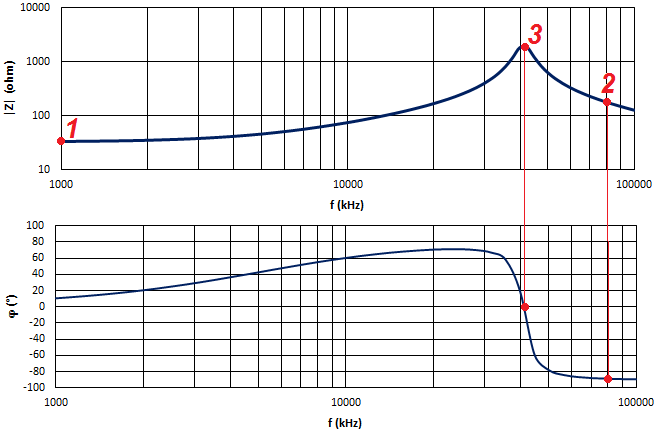
\includegraphics[scale=0.6]{obr06_prikladR.png}
		\end{center}
	\end{frame}
%------------------------------------------------------------------------------
	\begin{frame}
    \frametitle{Analysis Example}
		
		\begin{enumerate}
		\setcounter{enumi}{0}
			\item Resistance: $$R= 33\Omega$$
			\item Capacitance \textbf{(15 pF)}: $$C_p\approx \frac{1}{\omega \cdot \left|Z\right|}= \frac{1}{503\cdot 10^6\cdot180}= 11pF$$
			\item Inductance \textbf{(1 $\mu$H)}: $$L\approx Z_{RES}\cdot R \cdot C_p = 1900\cdot 33\cdot 15\cdot 10^{-12}= 940 nH$$
		\end{enumerate}
	\end{frame}
%------------------------------------------------------------------------------
%Frquency dependency of capacitors
%------------------------------------------------------------------------------
\section{\texorpdfstring{Frequency dependency of capacitors}{Frequency dependency of capacitors}}
%------------------------------------------------------------------------------
	\begin{frame}
    \frametitle{Equivalent Circuit}
		\begin{center}
		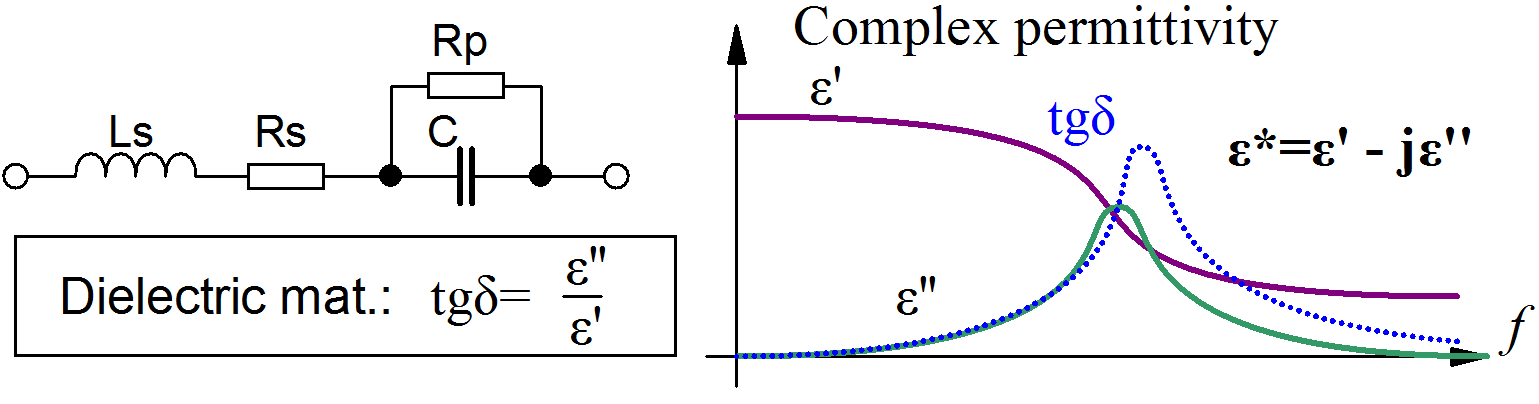
\includegraphics[scale=0.25]{obr07_ekvSchC.png}
		\end{center}
		\small
		Frequency dependence due to package properties:
		\begin{itemize}
			\item Parasitic inductance of the leads and electrodes $L_s$.
			\item Parasitic resistance of the leads $R_s$.
		\end{itemize}
		Frequency dependence due to material properties (complex permittivity):
		\begin{itemize}
			\item Change in dielectric power dissipation $R_p$ ($\epsilon ''$) - dissip. factor ($D$).
			\item Change in capacity $C$ ($\epsilon '$).
		\end{itemize}
	\end{frame}
%------------------------------------------------------------------------------
	\begin{frame}
    \frametitle{Technology Overview}
		
		\begin{itemize}
			\item Capacitors with higher capacitance have lower resonant frequency.
			\item Foil capacitors have larger parasitic inductance $L_s$.
			\item Electrolytic capacitors have higher serial parasitic resistance $R_s$ due to electrolyte presence.
			\item Equivalent scheme of electrolytic capacitor:
		\end{itemize}
		\begin{center}
		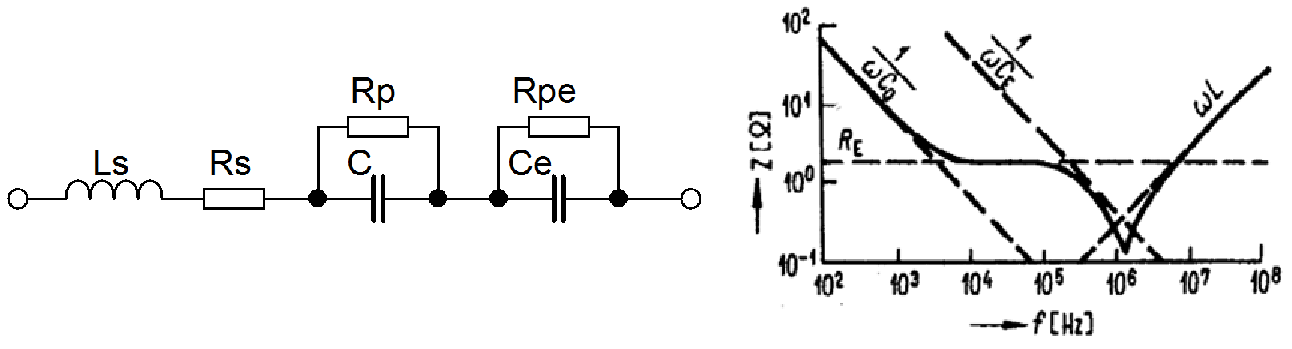
\includegraphics[scale=0.3]{obr08_ekvSchCe.png}
		\end{center}
	\end{frame}
%------------------------------------------------------------------------------
	\begin{frame}
    \frametitle{Impedance Plot Example}

		\begin{center}
			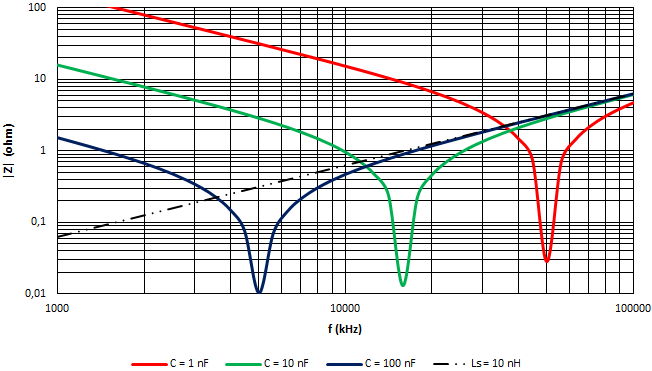
\includegraphics[scale=0.62]{obr03_impedanceC.png}
		\end{center}
	\end{frame}
%------------------------------------------------------------------------------
	\begin{frame}
    \frametitle{Equivalent Circuit Analysis}
		Impedance: 
		$$\hat{Z}= R_s+\frac{R_p}{\left(1+(\omega C R_p)^2\right)} + j\left(\omega L_s -\frac{1}{\omega C} \cdot \frac{(\omega C Rp)^2}{\left(1+(\omega C R_p)^2\right)}\right)$$
		Low frequencies ($\omega << \omega_{RES}$): \textcolor{red}{capacitance}
		$$\hat{Z}\approx \frac{1}{j\omega C}$$
		High frequencies ($\omega >> \omega_{RES}$): \textcolor{red}{parasitic inductance}
		$$\hat{Z}\approx j\omega L_s$$
	\end{frame}
%------------------------------------------------------------------------------
	\begin{frame}
    \frametitle{Equivalent Circuit Analysis - Resonance}
		Resonance frequency:
		$$\omega_{RES}= \sqrt{\frac{1}{L_sC} - \left(\frac{1}{R_pCp}\right)^2}\approx \sqrt{\frac{1}{L_sC}}$$
		Impedance at $\omega_{RES}$
		$$\hat{Z}_{RES}=R_s + \frac{Z_0^2}{R_p}\approx R_s$$
		\small
		\begin{itemize}
			\item The approximation is made for capacitors with high resistance $R_p$ and value of capacitance $C>$ 1 $nF$
			\item The higher resistance at the resonance is caused by the factor $\frac{Z_0^2}{R_p}$ or by \textbf{skin-effect}. 
			\item The parasitic resistances can change due to frequency dependence of complex permittivity.
		\end{itemize}
	\end{frame}
%------------------------------------------------------------------------------
	\begin{frame}
    \frametitle{Analysis Example}
		
		\begin{center}
			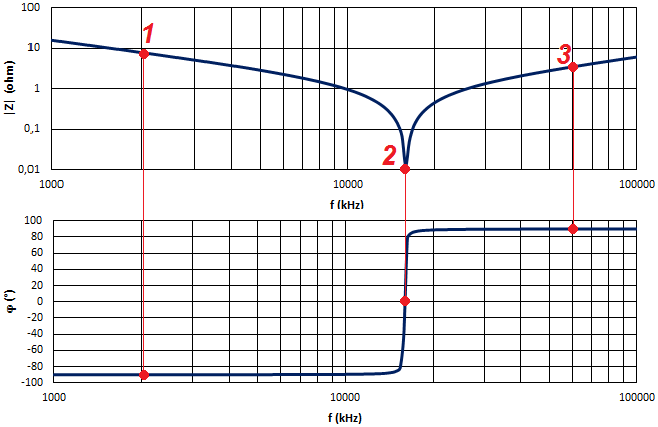
\includegraphics[scale=0.6]{obr09_prikladC.png}
		\end{center}
	\end{frame}
%------------------------------------------------------------------------------
	\begin{frame}
    \frametitle{Analysis Example}
		
		\begin{enumerate}
		\setcounter{enumi}{0}
			\item Capacitance \textbf{(10 nF)}: $$C\approx \frac{1}{\omega \cdot \left|Z\right|}= \frac{1}{12.6\cdot 10^6\cdot7.85}= 10.1 nF$$
			\item Serial resistance \textbf{0.01 $\Omega$)}: $$R_s \approx Z_{RES} = 0.01\Omega$$
			\item Inductance \textbf{(10 nH)}: $$L\approx \frac{\left|Z\right|}{\omega}= \frac{3.65}{376\cdot 10^6}= 9.7 nH$$
		\end{enumerate}
	\end{frame}
%------------------------------------------------------------------------------
%Frquency dependency of inductors
%------------------------------------------------------------------------------
\section{\texorpdfstring{Frequency dependency of inductors}{Frequency dependency of inductors}}
%------------------------------------------------------------------------------
	\begin{frame}
    \frametitle{Equivalent Circuit}
		\begin{center}
		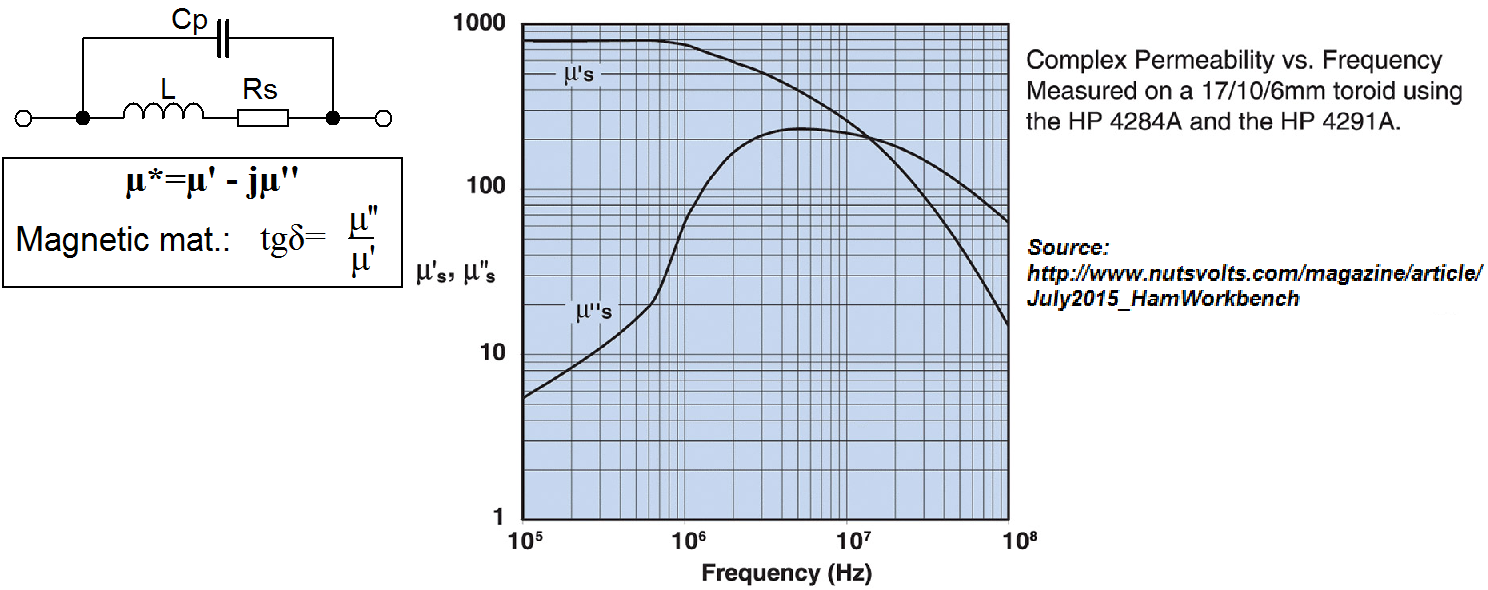
\includegraphics[scale=0.25]{obr10_ekvSchL2.png}
		\end{center}
    
		\begin{itemize}
			\item The same equivalent circuit as in case of resistors.
			\item The frequency dependence strongly affected by core material properties and skin-effect.
			\item Coils with high impedance have lower resonant frequencies.
		\end{itemize}
	\end{frame}
%------------------------------------------------------------------------------
	\begin{frame}
    \frametitle{Impedance Plot Example}

		\begin{center}
			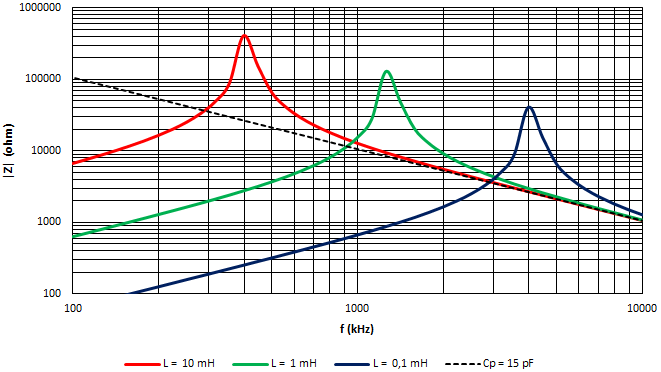
\includegraphics[scale=0.61]{obr04_impedanceL.png}
		\end{center}
	\end{frame}
%------------------------------------------------------------------------------
	\begin{frame}
    \frametitle{Equivalent Circuit Analysis}
		Very low frequencies ($\omega \rightarrow 0$): \textcolor{red}{parasitic resistivity}
		$$\hat{Z}\approx R_s$$
		Low frequencies ($\omega << \omega_{RES}$): \textcolor{red}{inductance}
		$$\hat{Z}\approx j\omega L$$
		High frequencies ($\omega >> \omega_{RES}$): \textcolor{red}{parasitic capacitance effect}
		$$\hat{Z}\approx \frac{1}{j\omega C_p}$$
	\end{frame}
%------------------------------------------------------------------------------
	\begin{frame}
    \frametitle{Analysis Example}
		
		\begin{center}
			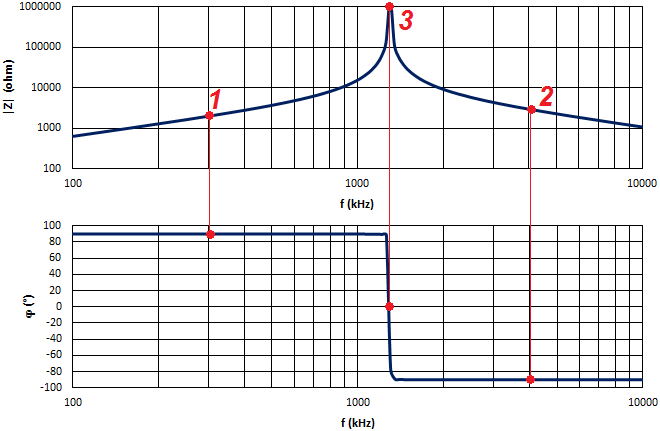
\includegraphics[scale=0.6]{obr11_prikladL.png}
		\end{center}
	\end{frame}
%------------------------------------------------------------------------------
	\begin{frame}
    \frametitle{Analysis Example}
		
		\begin{enumerate}
		\setcounter{enumi}{0}
			\item Inductance \textbf{(1 mH)}: $$L\approx \frac{\left|Z\right|}{\omega}= \frac{2050}{1885\cdot 10^3}= 1.1 mH$$
			\item Parallel capacitance \textbf{(15 pF)}: $$C\approx \frac{1}{\omega \cdot \left|Z\right|}= \frac{1}{25.1\cdot 10^6\cdot2970}= 13 pF$$
			\item Serial resistance \textbf{10 $\Omega$)}: $$R_s \approx \frac{Z_0^2}{Z_{RES}}=\frac{10^{-3}}{15\dot 10^{-12}\cdot 10^6}= 6.67 \Omega$$
			
			\begin{itemize}
				\item \large\textbf{\textcolor{red}{NO!}} \small... better to find out the serial resistance from DC measurement.
			\end{itemize}
		\end{enumerate}
	\end{frame}
%------------------------------------------------------------------------------
%Notes
%------------------------------------------------------------------------------
\section{\texorpdfstring{Notes}{Notes}}
%------------------------------------------------------------------------------
\begin{frame}
    \frametitle{NOTES}
		\small
	\begin{itemize}
		\item In case of impedance plot use logarithmic scale for both axis.
		\item In case of phase plot use logarithmic scale only for frequency.
		\item $$\hat{Z} = R + jX$$
		\item $$\left|Z\right|= \sqrt{R^2 + X^2}$$
		\item $$\varphi = arctg \frac{X}{R}$$
		\item resonance: $X = 0$, $\varphi = 0$, parallel $\Rightarrow$ high $\left|Z\right|$, serial $\Rightarrow$ low $\left|Z\right|$
	\end{itemize}
	\end{frame}

%------------------------------------------------------------------------------
\end{document}